\newthought{\textbf{Adjie Yusmunandar - 2020903430005 - TRKJ 3B}}


\newday{\textbf{1 - 2 Desember 2022} - Instalasi dan Konfigurasi Apache Hadoop}
\begin{enumerate}
\item Kendala dan Solusi \\
Kendala :\\
Saat melakukan penginstalan hadoop terdapat masalah pada saat mengecek hadoop version dan  pada saat melakukan konfigurasi hadoop terdapat kendala pada saat melakukan hdfs namenode -format. Perintah ini tidak mau dijalankan karena ada kesalahan dalam penulisan pada file yarn-site.xml.

Solusi :\\
Melakukan perubahan penulisan pada file yarn-site.xml,

\item Kesimpulan
\newline
 penginstalan hadoop dan konfigurasi hadoop berhasil dijalankan sesuai perintah-perintah yang ada.

\begin{figure}
\setlength{\belowcaptionskip}{-10pt}
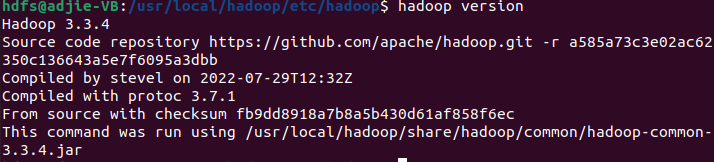
\includegraphics[width=\textwidth]{Adjie Yusmunandar/instalasi hadoop}
\caption{Versi hadoop yang Terinstall}
\label{gam:hasil instalasi apache hadoop}
\end{figure}

\begin{figure}
\setlength{\belowcaptionskip}{-10pt}
\includegraphics[width=\textwidth]{Adjie Yusmunandar/konfigurasi hadoop}
\caption{Versi hadoop yang Terinstall}
\label{gam:hasil konfigurasi hadoop}
\end{figure}
\end{enumerate}

\newday{\textbf{2 Desember 2022}}
\begin{enumerate}
\item Kendala dan Solusi
% jelaskan kendala dan penyebab yang dialami saat mengikuti praktikum serta solusi atau langkah-langkah yang telah dilakukan

\item Kesimpulan
% berikan kesimpulan dari praktikum yang telah dikerjkan

\end{enumerate}

\newday{\textbf{8 Desember 2022}}
\begin{enumerate}
\item Kendala dan Solusi
% jelaskan kendala dan penyebab yang dialami saat mengikuti praktikum serta solusi atau langkah-langkah yang telah dilakukan

\item Kesimpulan
% berikan kesimpulan dari praktikum yang telah dikerjkan

\end{enumerate}

\newday{\textbf{9 Desember 2022}}
\begin{enumerate}
\item Kendala dan Solusi
% jelaskan kendala dan penyebab yang dialami saat mengikuti praktikum serta solusi atau langkah-langkah yang telah dilakukan

\item Kesimpulan
% berikan kesimpulan dari praktikum yang telah dikerjkan

\end{enumerate}

\newday{\textbf{15 Desember 2022}}
\begin{enumerate}
\item Kendala dan Solusi
% jelaskan kendala dan penyebab yang dialami saat mengikuti praktikum serta solusi atau langkah-langkah yang telah dilakukan

\item Kesimpulan
% berikan kesimpulan dari praktikum yang telah dikerjkan

\end{enumerate}

\newday{\textbf{16 Desember 2022}}
\begin{enumerate}
\item Kendala dan Solusi
% jelaskan kendala dan penyebab yang dialami saat mengikuti praktikum serta solusi atau langkah-langkah yang telah dilakukan

\item Kesimpulan
% berikan kesimpulan dari praktikum yang telah dikerjkan

\end{enumerate}

\newday{\textbf{22 Desember 2022}}
\begin{enumerate}
\item Kendala dan Solusi
% jelaskan kendala dan penyebab yang dialami saat mengikuti praktikum serta solusi atau langkah-langkah yang telah dilakukan

\item Kesimpulan
% berikan kesimpulan dari praktikum yang telah dikerjkan

\end{enumerate}


